\documentclass[12pt,a4paper,leqno]{report}

\usepackage[ansinew]{inputenc}
\usepackage[T1]{fontenc}
\usepackage[finnish]{babel}
\usepackage{amsthm}
\usepackage{amsfonts}         
\usepackage{amsmath}
\usepackage{amssymb}


\usepackage{mathtools}
\usepackage{algorithmic}
\usepackage{tikz}
\usepackage{pgfplots}
\pgfplotsset{%
  colormap={whitered}{color(0cm)=(white);
  color(1cm)=(orange!75!red)}
}
\usetikzlibrary{arrows,automata}
%\usepackage[style=numeric]{biblatex}
%\addbibresource{sources.bib}

%hallitse tilaa ennen kappale otsikkoa
\usepackage{etoolbox}
\makeatletter
\patchcmd{\@makechapterhead}{\vspace*{50\p@}}{}{}{}% Removes space above \chapter head
\patchcmd{\@makeschapterhead}{\vspace*{50\p@}}{}{}{}% Removes space above \chapter* head
\makeatother

\newcommand{\pr}{\textbf{P}}

\newcommand{\R}{\mathbb{R}}
\newcommand{\C}{\mathbb{C}}
\newcommand{\Q}{\mathbb{Q}}
\newcommand{\N}{\mathbb{N}}
\newcommand{\No}{\mathbb{N}_0}
\newcommand{\Z}{\mathbb{Z}}
\newcommand{\diam}{\operatorname{diam}}

\theoremstyle{plain}
\newtheorem{lause}[equation]{Lause}
\newtheorem{lem}[equation]{Lemma}
\newtheorem{prop}[equation]{Propositio}
\newtheorem{kor}[equation]{Korollaari}

\theoremstyle{definition}
\newtheorem{maar}[equation]{M��ritelm�}
\newtheorem{konj}[equation]{Konjektuuri}
\newtheorem{esim}[equation]{Esimerkki}
\newtheorem{merk}[equation]{Merkint�}


\theoremstyle{remark}
\newtheorem{huom}[equation]{Huomautus}

\pagestyle{plain}
\setcounter{page}{1}
\addtolength{\hoffset}{-1.15cm}
\addtolength{\textwidth}{2.3cm}
\addtolength{\voffset}{0.45cm}
\addtolength{\textheight}{-0.9cm}

\title{kandi ty�otsikkko}
\author{Topias Karjalainen}
\date{\today}


\begin{document}

\maketitle

\tableofcontents

\chapter{Johdanto}\label{johd}




\chapter{Teoriaa}\label{teor}

\section{Perusm��ritelmi�}

M��ritell��n ensiksi todenn�k�isyys.

\begin{maar}
	\textit{$\sigma$-algebra.} Olkoot $\Omega$ mielivaltainen ep�tyhj� joukko. Sigma-algebra perusjoukolla $\Omega$ on sen osajoukkojen joukkoperhe $\mathcal{F}$, joka toteuttaa ehdot:
	
	\begin{enumerate}
		\item $\emptyset\in\mathcal{F}$
		\item jos $A\in\mathcal{F},\ niin\ A^c \in\mathcal{F}$
		\item jos jos $A_k\in\mathcal{F},\ kaikilla\ k\in K$, miss� $K$ on numeroituva joukko, niin $\bigcup_{k\in K} A_k \in \mathcal{F}$
	\end{enumerate}
\end{maar}

\begin{maar}
	Kuvaus \pr\ liitt�� kuhunkin tapahtumaan $A$ \textit{todenn�k�isyyden}, joka on luku suljetulla v�lill� [0,1] ja sille p�tee:
	\begin{enumerate}
		\item $\pr(\Omega)=1$
		\item Jos $A$ on tapahtuma, niin sen komplementtitapahtuman $A^c$ todenn�k�isyys on $\pr(A^c)= 1 - \pr(A)$
		\item Jos $(A_k)_{k\in\N}$ ovat erillisi� tapahtumia, niin 
		\begin{displaymath}
			\pr(\bigcup_{k\in\N} A_k) = \sum_{k\in\N}\pr(A_k)
		\end{displaymath}
	\end{enumerate}
\end{maar}

\begin{maar}
	Kolmikkoa $(\Omega, \mathcal{F}, \pr )$ kutsutaan \textit{todenn�k�isyysavaruudeksi}.
\end{maar}

\begin{maar}
	\textit{Satunnaismuuttuja} $X$ on (l�hes) mielivaltainen kuvaus $X:\Omega\rightarrow S$, jossa $S$ on \textit{tilajoukko}. 
\end{maar}

\section{Markovin ketjut}

\subsection{��rellinen tilajoukko}

\begin{maar}
	Jono $(X_n:n=1,2,3,...)$ satunnaismuuttujia on diskreettiaikainen \textit{stokastinen prosessi}.
\end{maar}

\begin{merk}
	Merkit��n stokastista prosessia merkinn�ll� $\{ X_n \}$
\end{merk}

\begin{maar}
	Stokastinen prosessi $\{X_n\}$ on \textit{Markovin ketju}, jos kaikilla alkuhetkill� $m,n$ ja tiloilla $i,j\in S$ on voimassa
	\begin{equation}\label{markov-property}
		\begin{split}
			&\pr(X_{n+1}=j|X_0=i_0,X_1=i_1,...,X_{n-1}=i_{n-1},X_n=i) \\
		 &= \pr(X_{n+1}=j|X_n=i) 
		\end{split}
	\end{equation}
	ja \textit{siirtym�todenn�k�isyyksille} on voimassa 
	\begin{equation}\label{stationary}
		p_{ij}=\pr(X_{n+1}=j|X_n=i)=\pr(X_{m+1}=j|X_m=i)
	\end{equation}
	Yht�l�� \ref{markov-property} kutsutaan \textit{Markovin-ehdoksi} ja yht�l�� \ref{stationary} taas kutsutaan \textit{stationarisuusehdoksi}, mik� tarkoittaa, 
	ett� siirtym�todenn�k�isyys tilojen $i\ \text{ja}\ j$ v�lill� ei riipu ajasta $m\ \text{ja}\ n$, vaan pelk�st��n tiloista $i\ \text{ja}\ j$.
\end{maar}

\begin{maar}
	Satunnaismuuttujan $X_0$ jakaumaa kutsutaan \textit{alkujakaumaksi}. 
\end{maar}

\begin{lause}
	Ajanhetkell� $n\geq 1$ polun $(i_0,...i_n)$ todenn�k�isyys on 
	\begin{equation}
		\pr (X_0=i_0,...,X_n=i_n) = p_{i_0} p_{i_0,i_1} p_{i_1,i_2} ... p_{i_{n-1},i_n}
	\end{equation} 
\end{lause}
\begin{proof}
	K�ytt�en ehdollisen todenn�k�isyyden kaavaa, saadaan 2:lle tapahtumalle
	\begin{equation*}
		\pr (A_0, A_1)=\pr(A_0)\pr(A_1|A_0)
	\end{equation*}
	Jos tapahtumia on kolme, saadaan
	\begin{equation*}
		\pr (A_0, A_1, A_2)=\pr(A_0)\pr(A_1|A_0)\pr(A_2|A_1, A_0)
	\end{equation*}
	nelj�
	\begin{equation*}
		\pr (A_0, A_1, A_2, A_3)=\pr(A_0)\pr(A_1|A_0)\pr(A_2|A_1, A_0)\pr(A_3|A_2,A_1,A_0)
	\end{equation*}
	ja n
	\begin{equation}\label{condprob}
		\pr (A_0,...,A_n)=\pr(A_0)\pr(A_1|A_0)...\pr(A_n|A_{n-1},...A_0)
	\end{equation}
	T�m� on yleinen ehdollinen todenn�k�isyys. Merkataan $A_n \coloneqq (X_i=i_n)$. Koska k�sittelemme Markovin ketjua, niin yht�l� \ref{markov-property} p�tee, jolloin yht�l�st� \ref{condprob} saadaan 
	\begin{equation*}
		\pr(X_0=i_0,...,X_n=i_n) = \pr(X_0=i_0) \pr(X_1=i_1|X_0=i_0)...\pr(X_n=i_n|X_{n-1}=i_{n-1})
	\end{equation*}
	jossa $\forall n=0,1,2,...,n: \pr(X_n=i_n|X_{n-1}=i_{n-1})$ on siirtym�t�denn�k�isyys $p_{i_{n-1},i_n}$ jolloin tulos seuraa substituoimalla termit.
\end{proof}

\begin{merk}
	\begin{equation}
		p_{ij}^{(m)} \coloneqq \pr (X_m=j|X_0=i),\ i,j\in S,m\in T
	\end{equation}
	on siirtym�todenn�k�isyys tilasta $i$ tilaan $j$, kun aikaa kuluu $m$ yksikk��.
\end{merk}

\begin{maar}
	\textit{Siirtym�matriisi} on matriisi
	\begin{equation}
		\pr ^{(m)} \coloneqq (p_{ij}^{(m)})_{i,j} =
		\begin{pmatrix}
			p_{00}^{(m)} & p_{01}^{(m)} & \dots & p_{0n}^{(m)} \\
			p_{10}^{(m)} & p_{11}^{(m)} & \dots & p_{1n}^{(m)} \\
			\vdots & & \ddots & \vdots \\
			p_{n0}^{(m)} & p_{n1}^{(m)} & \dots & p_{nn}^{(m)}
		\end{pmatrix}
	\end{equation}
\end{maar}

\begin{lause}
	Kaikilla ajanhetkill� on voimassa
	\begin{equation}
		\pr ^{(m)} = \pr ^m
	\end{equation}
\end{lause}
\begin{proof}
	Todistus on melko pitk�, joten ohitetaan se.
\end{proof}

\begin{maar}
	Todenn�k�isyysjakauma $\pi=(\pi)_{i\in S}$ on Markovin ketjun $\{X_n\}$ tasapainojakauma, jos 
	\begin{equation}\label{stationary-dist}
		\sum_{i\in S} \pi_i p_{ij}=\pi_j, \forall j\in S
	\end{equation}
	Yht�l� \ref{stationary-dist} voidaan kirjoittaa my�s muotoon 
	\begin{equation}\label{stationary-dist2}
		\pi^T\pr= \pi^T
	\end{equation}
\end{maar}

\begin{lause}
	��rellisell� Markovin ketjulla on aina jokin tasapainojakauma $\pi$.
\end{lause}

\begin{maar}\label{kaant-disk}
	Markovin ketju on \textit{k��ntyv�}, jos l�ytyy sellainen TN-jakauma $\lambda=(\lambda_i)_{i\in S}$, ett� 
	\begin{equation}
		\lambda_ip_{ij}= \lambda_jp_{ji},\forall i,j\in S
	\end{equation}
\end{maar}

\begin{lause}
	Jos Markovin ketju on k��ntyv�, niin $\lambda=\pi$ on sen tasapainojakauma.
\end{lause}

\begin{esim}
	Pohditaan lyhytt� esimerkki�, jossa tilajoukko on $S=\{"sataa", "paistaa"\}$. M��ritell��n siirtym�todenn�k�isyydet siirtym�matriisilla
	\begin{displaymath}
		\pr ^{(1)}=  
		\begin{pmatrix}
			0.7 & 0.3 \\
			0.2 & 0.8
		\end{pmatrix}
	\end{displaymath}
	T�m� voidaan visualisoida seuraavanlaisesti:
	
	\begin{center}
		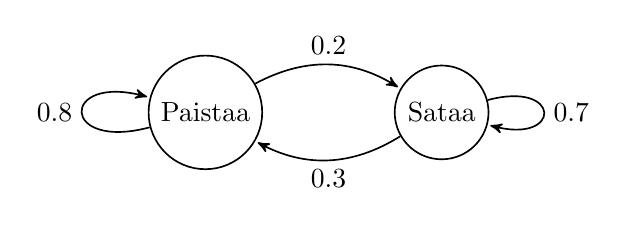
\begin{tikzpicture}[->,>=stealth',shorten >=1pt,auto,node distance=3cm,semithick]

		\node[state](s){Paistaa};
    	\node[state, right of=s](r){Sataa};
		\draw[every loop]
            (s) edge[bend left] node {0.2} (r)
            (r) edge[bend left] node {0.3} (s)
            (r) edge[loop right] node {0.7} (r)
            (s) edge[loop left] node {0.8} (s);
	\end{tikzpicture}
	\end{center}
	Ketju on ��rellinen, joten sill� on tasapainojakauma. Yht�l� \ref{stationary-dist2} implikoi, ett� jakauma $\pi$ on siirtym�matriisin $\pr$ vasen ominaisvektori ($\pi^T\pr=\lambda\pi^T$, jossa $\lambda=1$). T�m� voidaan ratkaista numeerisesti, ja ratkaisu on $\pi^T=(0.4, 0.6)$. Helposti nyt n�hd��n, ett� \ref{stationary-dist2} p�tee.
\end{esim}

\subsection{��ret�n jatkuva tilajoukko}
Kun Markovin ketjun tilajoukko $S$ ei olekkaan rajattu (esimerkiksi, jos halutaan simuloida normaalijakaumasta, joka voi saada mink� vain arvon v�lilt� $(-\infty,\infty)$), niin teoria muuttuu hieman. Suurin osa tuloksista p�tee pienin muutoksin, mutta niiden todistaminen on hankalaa ja ylitt�� kanditason. Esitet��n kuitenkin tarvittavat perustulokset.


\begin{maar}
	Kun $S$ on rajoittamaton, siirtym�matriisi on parasta ajatella kuvauksena $T: S\times S \rightarrow [0,1]$, joka kuvaa tilaparin $x,y\in S$ todenn�k�isyydeksi $T(x,y)$
\end{maar}

\begin{maar}
	Iistym�todenn�k�isyys $p^{(n)}_{ij}$ voidaan kirjoittaa \textit{siirtym�tiheyten�} $T^{(n)}(x,y)$, jolle p�tee
	\begin{equation}\label{siirt-tiheys}
		\int_S T(x,y)dy = 1 \hspace{1cm} \text{ja} \hspace{1cm} \int_S T^{(n)}(x,y)dy = 1, \forall n \geq 1
	\end{equation}
\end{maar}

\begin{maar}
	Jakauma $\pi$ on Markovin ketjun $\{ X_n \}$ kun $S$ on jatkuva, tasapainojakauma jos 
	\begin{equation}
		\pi(y) = \int_S \pi(x) T(x,y) dx
	\end{equation}
\end{maar}

\begin{maar}\label{kaant-jatk}
	Markovin ketju jatkuvassa $S$:ss� on k��ntyv�, jos on olemassa 
	\begin{equation}
		\pi(x)T(x,y)=\pi(y)T(y,x), \forall x,y\in S
	\end{equation}
\end{maar}

\begin{lause}
	Jos Markovin ketju $\{X_n\}$ on k��ntyv� ja tilajoukko $S$ on jatkuva, niin $\pi$ on sen tasapainojakauma.
\end{lause}

\begin{proof}
	Yht�l�n \ref{siirt-tiheys} mukaan $\int_S T(y,x)dx = 1$, joten
	\begin{equation}
		\int_S \pi(x) T(x,y) dx = \int_S \pi(y) T(y,x) dx = \pi(y)\int_S T(y,x) dx = \pi(y)
	\end{equation}
\end{proof}

























































\chapter{Metropolis--Hastings algoritmi}

\textit{Metropolis--Hastings} algoritmi on kehittelij�idenss� Nicholas Metropolisksen (1915-1999) ja \textit{Wilfred Keith Hastings}:n (1930-2016) mukaan nimetty MCMC-menetelm�, jolla voidaan simuloida Bayesil�isess� analyysissa k�ytett�vi� posteriori jakaumia my�s silloin kun tiheys on mahdotonta m��ritt�� analyyttisesti.

\begin{maar}\label{mh-maar}
	Metropolis--Hastings algoritmi on seuraavanlainen
	\begin{enumerate}
		\item Valitaan aloitus tila $\theta_0$ ja asetetaan $t=0$
		\item Generoidaan kandidaatti tila $\theta'$ satunnaisesti jakaumasta $J_n(\theta'|\theta_{n-1})$
		\item Lasketaan tiheyksien tai todenn�k�isyyksien suhde
		\begin{displaymath}
			r = \frac{p(\theta'|y)/J_n(\theta'|\theta_{n-1})}{p(\theta_{n-1}|y)/J_n(\theta_{n-1}|\theta')}
		\end{displaymath}
		\item Asetetaan
		\begin{displaymath}
			\theta_t= 
			\begin{cases}
				\theta', \text{todenn�k�isyydell�} \hspace{0.3cm} \min(r,1) \\
				\theta_{t-1}, \text{muuten}
			\end{cases}
		\end{displaymath}
	\end{enumerate}
	Jossa $J_t(\theta'|\theta^{t-1})$ on ns. ehdotusjakauma (eng. proposal distribution).
\end{maar}

\begin{lause}
	M��ritelm�n \ref{mh-maar} algoritmi tuottaa Markovin ketjun jolla on uniikki tasapainojakauma, ja jonka tasapainojakauma on posteriorijakauma $p(\theta|y)$, jossa $y$ on data. 
\end{lause}

\begin{proof}
	Ohitamme todistuksen, ett� kyseess� Markovin ketju jolla yksi tasapainojakauma, mutta todistamme toisen osan, eli ett� tasapainojakauma on haluttu $p(\theta|y)$ eli posteriori jakauma. Todistus nojautuu Markovin ketjun k��ntyvyysominaisuuteen (\ref{kaant-disk} ja \ref{kaant-jatk}), eli
	\begin{equation}\label{kaant-mcmc}
		T(\theta_{n+1}|\theta_n)p(\theta_n|y) = T(\theta_n|\theta_{n+1})p(\theta_{n+1}|y)
	\end{equation}
	joka on siis riitt�v� ehto tasapainojakauman olemassaololle. Mietit��n kahta tapausta: (1) $\theta_n \neq \theta_{n-1}$ ja (2) $\theta_n = \theta_{n-1}$.
	Tapauksen (2) siirtym� voi tapahtua kahdella tavalla. Joko kohdassa 4. ehdotus $\theta'$ hyl�t��n, tai se hyv�ksyt��n, mutta osutaan sattumanvaraisesti takaisin samaan kohtaan. Kuitenkin selv�sti n�hd��n, ett� ehto \ref{kaant-mcmc} p�tee tilanteessa (2).
	
	Tilanteessa (1)
\end{proof}



\begin{thebibliography}{9}

%\bibitem{ET}
%Gustav Elfving ja Pekka Tuominen: Todenn�k�isyyslaskenta II, 2.\ painos, Limes ry, 1990.
%
%\bibitem{Hol}
%Ilkka Holopainen: Mitta ja integraali, luentomoniste, Helsingin yliopisto, 2004.
%
%\bibitem{Ros}
%Sheldon Ross: A First Course in Probability, 5th edition, Prentice-Hall, 1998.
%
%\bibitem{Tuo}
%Pekka Tuominen: Todenn�k�isyyslaskenta I, 5.\ painos, Limes ry, 2000.

\end{thebibliography}

\end{document}
